\subsection{Wat is netwerkbeveiliging}
We kunnen de volgende wenselijke eigenschappen van veilige communicatie identificeren:
\begin{itemize}
    \item \textcolor{red}{\textbf{Confidentialiteit}}: enkel de afzender en beoogde ontvanger zou de inhoud van het verzonden bericht kunnen begrijpen. Het is noodzakelijk dat het bericht op een manier geëncrypteerd is zodat het onderschepte bericht niet begrepen kan worden door een onderschepper.(Verzender encrypteerd bericht, ontvanger decrypteerd bericht.)
    \item \textcolor{red}{\textbf{Authenticatie}}: de zender en ontvanger willen de identiteit van elkaar bevestigen.
    \item \textcolor{red}{\textbf{Bericht integriteit:}} de zender en ontvanger willen zeker zijn dat de inhoud van hun communicatie niet aangepast is.
    \item \textcolor{red}{\textbf{Operationele beveiliging (toegang en beschikbaarheid):}} diensten moeten toegankelijk en beschikbaar zijn voor gebruikers.
\end{itemize}

%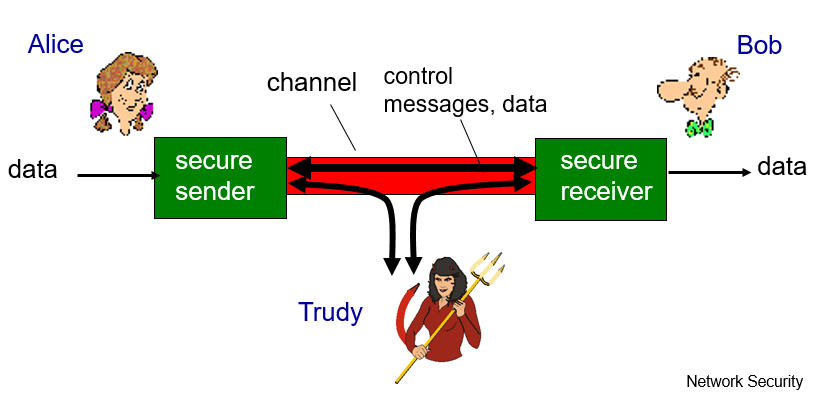
\includegraphics[width=0.30\textwidth]{./img/imghfdst8/hfdst8puntje1.png}\\[1cm]
\begin{figure}[h]
    \centering
    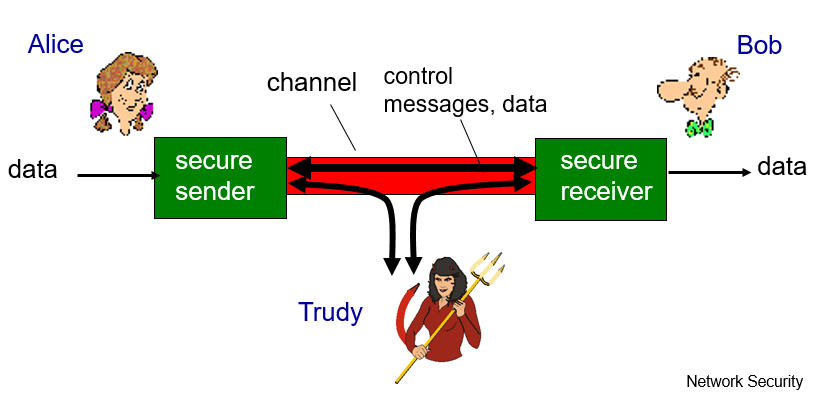
\includegraphics[width=7in]{./img/imghfdst8/hfdst8puntje1.png}
    \caption{Netwerkbeveiliging }      
    \label{fig:Netwerkbeveiliging }
\end{figure}
%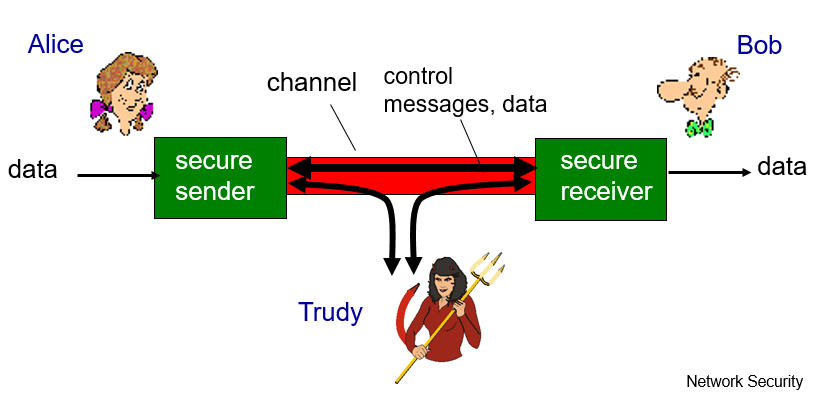
\includegraphics[width=7in]{./img/imghfdst8/hfdst8puntje1.png}\\[1cm]
\noindent Om data veilig uit te wisselen, gaan de zender en ontvanger controle en data berichten uitwisselen. Alle of sommige van deze berichten gaan geëncrypteerd zijn. 

\subsubsection{Een indringer kan volgende zaken uitvoeren:}

\begin{itemize}
    \item \textcolor{red}{\textbf{Afluisteren}}: sniffing en opnemen van controle- en data-berichten op het kanaal.
    \item \textcolor{red}{\textbf{Aanpassen}}, toevoegen of verwijderen van berichten of inhoud. 
    \item \textcolor{red}{Zich als een ander persoon voordoen}: kan valse (spoof) bronadres in packet steken (of elk ander veld in het packet)
    \item \textcolor{red}{\textbf{kapen/Hijacking}}: een lopende connectie overnemen door een zender of ontvanger te vervangen door zichzelf.
    \item \textcolor{red}{\textbf{Denial of service:}} voorkomen dat een dienst wordt gebruikt door anderen.
\end{itemize}